\documentclass[../ManualeSviluppatore.tex]{subfiles}

\begin{document}
\section{Persistenza dei dati}
\label{sec:PersistenzaDeiDati}

	\subsection{Database locale e remoto}
		L'applicazione è costituita da un database locale in SQLite che in base alle necessità dell'utente si sincronizza con quello remoto in PostgreSQL attraverso un RESTful server. Il database contiene tutti i dati necessari a comporre i grafi degli edifici supportati. L'applicazione, ossia la parte client della comunicazione, effettua solo richieste GET dal server, nessun'altra operazione può essere effettuata (DELETE, POST e PUT) dall'applicazione. 
	
		\subsection{Diagramma ER}
			Di seguito si descrive il Diagramma ER della base di dati rappresentato in figura \ref{fig:Database}.
		\begin{figure} [p]
			\centering
				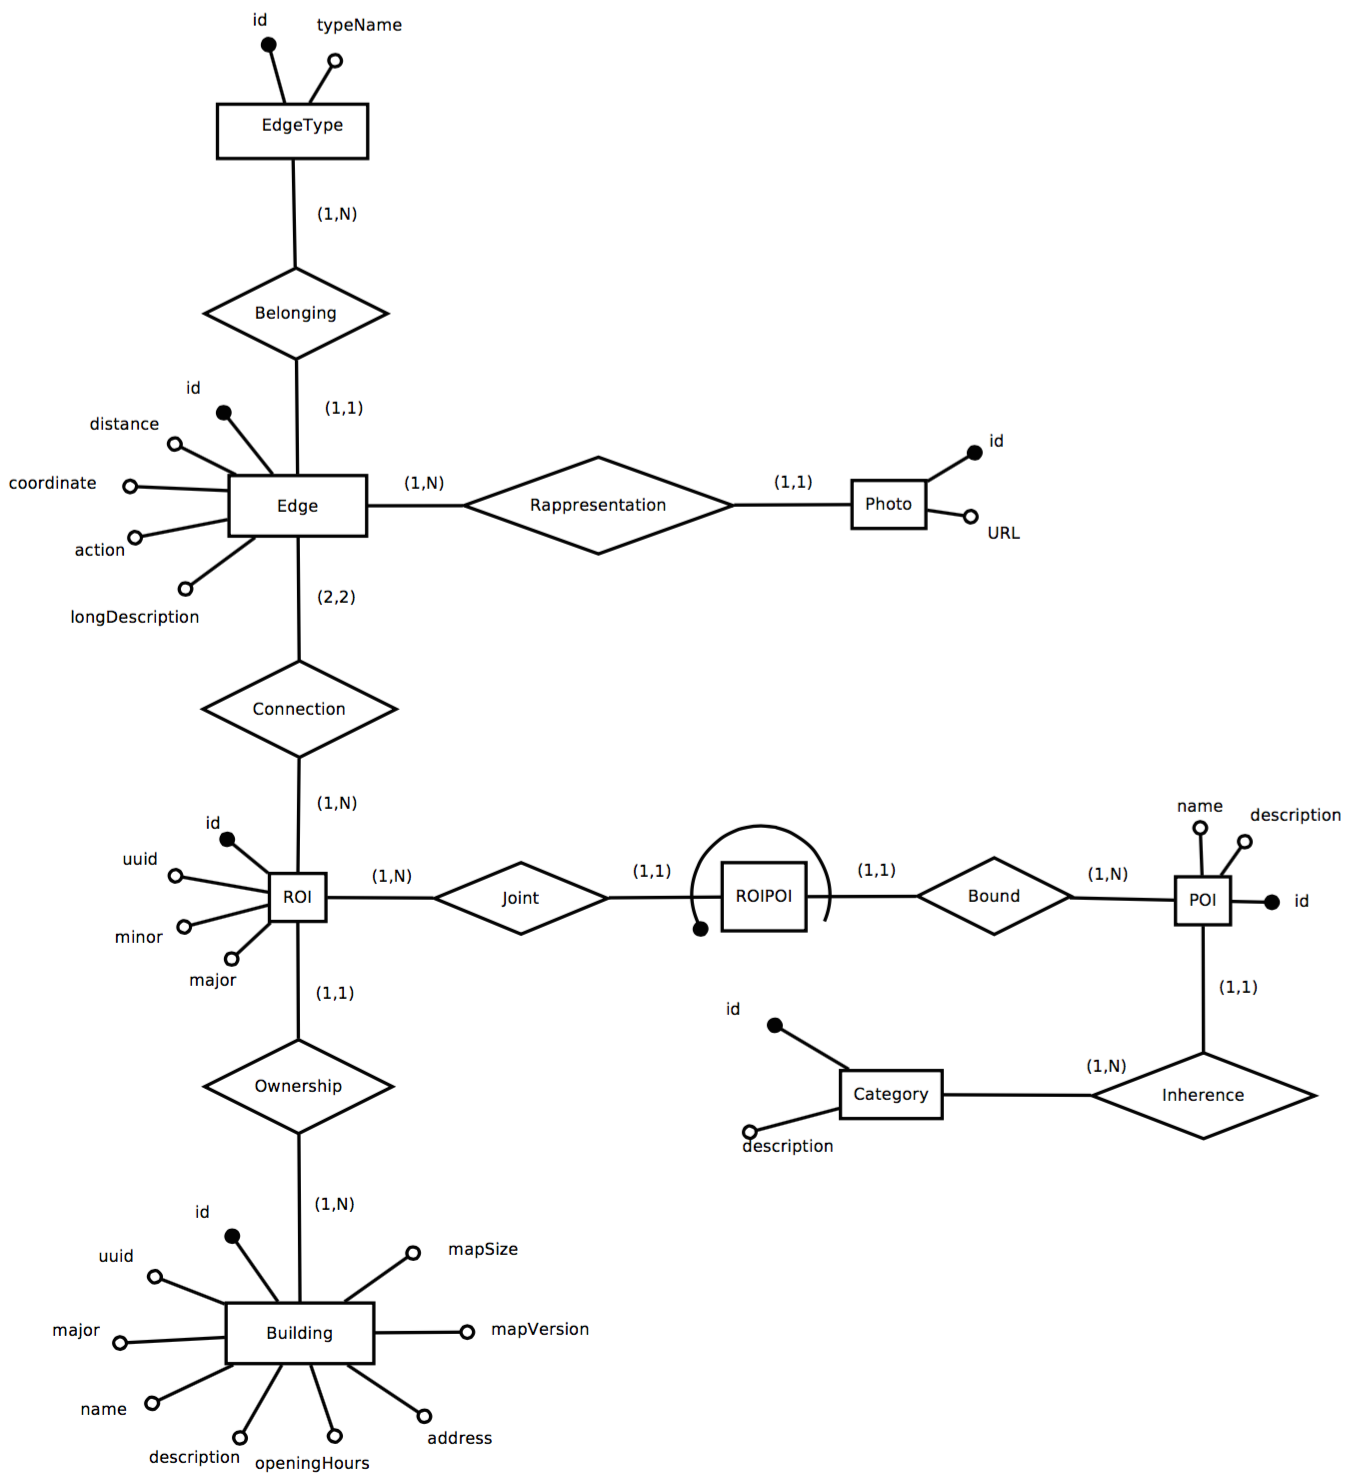
\includegraphics[width=\textwidth]{img/db}		
				\caption{Diagramma ER - Base di dati dell'applicazione}
				\label{fig:Database}
		\end{figure}
	\subsection{Descrizione relazioni}
		\subsubsection{Building}
		Relazione che contiene le informazioni degli edifici. Attributi:
		\begin{itemize}
			\item \textbf{id}: chiave primaria, intero;
			\item \textbf{uuid}: stringa, rappresenta l'identificativo UUID uguale per tutti i \gls{beacon} utilizzati dall'applicazione;
			\item \textbf{major}: intero, rappresenta l'identificativo Major uguali per tutti i \gls{beacon} di uno stesso edificio, chiave esterna verso la relazione Building;
			\item \textbf{name}: stringa, rappresenta il nome dell'edificio;
			\item \textbf{description}: stringa, rappresenta la descrizione dell'edificio e delle sue funzionalità;
			\item \textbf{openingHours}: stringa, rappresenta gli orari di apertura dell'edificio;
			\item \textbf{address}: stringa, rappresenta l'indirizzo dell'edificio;
			\item \textbf{mapVersion}: stringa, rappresenta la versione della mappa;
			\item \textbf{mapSize}: stringa, rappresenta la dimensione della mappa.
		\end{itemize}
		\subsubsection{ROI}
		Relazione che contiene le informazioni delle Region of interest. Attributi:
			\begin{itemize}
			\item \textbf{id}: chiave primaria, intero;
			\item \textbf{uuid}: stringa, rappresenta l'identificativo UUID uguale per tutti i \gls{beacon} utilizzati dall'applicazione;
			\item \textbf{major}: intero, rappresenta l'identificativo Major uguali per tutti i \gls{beacon} di uno stesso edificio;
			\item \textbf{minor}: intero, rappresenta l'identificativo Minor che identifica univocamente un \gls{beacon} in un edificio.
			\end{itemize}
		\subsubsection{ROIPOI}
		Relazione che contiene le associazioni tra Region of interest e Point of interest. Attributi:
			\begin{itemize}
			\item \textbf{idRoi}: intero, chiave esterna verso la relazione \gls{ROI};
			\item \textbf{idPoi}: intero, chiave esterna verso la relazione \gls{POI};
			\item chiave primaria (idRoi, idPoi).
			\end{itemize}
		\subsubsection{POI}
		Relazione che contiene le informazioni dei Point of interest. Attributi:
			\begin{itemize}
			\item \textbf{id}: chiave primaria, intero;
			\item \textbf{name}: string, rappresenta il nome associato al Point of interest;
			\item \textbf{description}: stringa, rappresenta la descrizione del Point of interest.
			\end{itemize}
		\subsubsection{Category}
		Relazione che contiene le informazioni delle categorie di Point of interest. Attributi:
			\begin{itemize}
			\item \textbf{id}: chiave primaria, intero;
			\item \textbf{description}: stringa, rappresenta la descrizione della categoria di Point of Interest.
			\end{itemize}
		\subsubsection{Edge}
		Relazione che contiene le informazioni delle connessioni tra le Region of interest, che rappresentano gli archi del grafo che rappresenta un edificio. Attributi:
			\begin{itemize}
			\item \textbf{id}: chiave primaria, intero;
			\item \textbf{distance}: intero, rappresenta la lunghezza dell'arco;
			\item \textbf{coordinate}: string, rappresenta l'ampiezza dell'arco che ha per lati l'arco e il collegamento tra la Region Of Interest di partenza e il nord polare; 
			\item \textbf{action}: string, rappresenta le azioni che bisogna compiere per superare l'arco;
			\item \textbf{longDescription}: string, rappresenta una descrizione dettagliata delle azioni che bisogna compiere per superare l'arco;
			\item \textbf{startROI}: intero, chiave esterna verso la relazione \gls{ROI}, rappresenta la Region of interest di partenza dell'arco;
			\item \textbf{endROI}: intero, chiave esterna verso la relazione \gls{ROI}, rappresenta la Region of interest di arrivo dell'arco.
			\end{itemize}
		\subsubsection{EdgeType}
		Relazione che contiene le informazioni sui tipi degli archi. Attributi:
			\begin{itemize}
			\item \textbf{id}: chiave primaria, intero;
			\item \textbf{typeName}: stringa, rappresenta la descrizione del tipo di arco.
			\end{itemize}
		\subsubsection{Photo}
		Relazione che contiene i link alle immagini associati ad un arco. Attributi:
			\begin{itemize}
			\item \textbf{id}: chiave primaria, intero;
			\item \textbf{URL}: stringa, rappresenta l'URL a cui recuperare l'immagine;
			\item \textbf{edgeId}: intero, chiave esterna verso la relazione Edge, rappresenta l'Edge a cui è associata l'immagine.
			\end{itemize}
	\subsection{Descrizione associazioni}
		\subsubsection{Ownership}
			Associazione che unisce ogni \gls{ROI} all'edificio di appartenenza.\\
			\textbf{Molteplicità}:(1,N) Ad ogni Building possono essere associati uno o più \gls{ROI}, ogni \gls{ROI} può essere associato un solo edificio.

		\subsubsection{Connection}
			Associazione che unisce ogni Edge ai \gls{ROI} di partenza e arrivo. \\
			\textbf{Molteplicità}:(2,N) Ad ogni Edge associa il \gls{ROI} di inizio e fine, ogni \gls{ROI}\ 
può essere associato ad uno o più Edge.

		\subsubsection{Joint}
			Associazione che unisce ogni \gls{ROI} ai ROIPOI di appartenenza. \\
			\textbf{Molteplicità}:(1,N) Ogni \gls{ROI} può essere associato ad uno o più ROIPOI, ogni ROIPOI può essere associato ad un unico \gls{ROI}.

		\subsubsection{Bound}
			Associazione che unisce ogni \gls{POI} ai ROIPOI di appartenenza. \\
			\textbf{Molteplicità}:(1,N) Ogni \gls{POI} può essere associato ad uno o più ROIPOI, ogni ROIPOI può essere associato ad un unico \gls{POI}.

		\subsubsection{Inherence}
			Associazione che unisce ogni \gls{POI} alla categoria a cui appartiene.\\
			\textbf{Molteplicità}:(1,N) Ogni \gls{POI} può essere associato ad una unica Category, ogni Category può essere associata a più \gls{POI}.

		\subsubsection{Rappresentation}
			Associazione che unisce ogni Photo all'Edge che rappresenta. \\
			\textbf{Molteplicità}:(1,N) Ogni Photo può essere associata ad un unico Edge, ogni Edge può avere più Photo.

		\subsubsection{Belonging}
			Associazione che unisce ogni Edge al tipo a cui appartiene.\\
			\textbf{Molteplicità}:(1,N) Ogni Edge può essere associato ad un unico EdgeType, ogni EdgeType può essere associato ad uno o più Edge.
		
	
	
	\subsection{Struttura oggetti Json}
	\label{sec:Json}
		La struttura di seguito proposta ricalca la struttura data agli oggetti JSON scaricati dal database remoto per l'installazione di mappe in locale. Nel caso in cui si voglia cambiare tale struttura si consiglia di estendere le classi con prefisso \textbf{Remote} e suffisso \textbf{Dao} presenti nel package \textbf{dao}.
	
	\subsubsection{Esempio di oggetto Json rappresentante una mappa}
			\begin{lstlisting}
{
  "building" : {
    "id" : 1,
    "uuid" : "f7826da6-4fa2-4e98-8024-bc5b71e0893e",
    "major" : 666,
    "name" : "Torre Archimede"
    "description" : "Edificio del Dipartimento di Matematica",
    "openingHours" : "08:00-19:00",
    "address" : "Via Trieste 63, 35121, Padova (PD)",
    "mapVersion" : "1.0",
    "mapVersion" : "5.2 KB"
  },
  "rois" : [ {
    "id" : 1,
    "uuid" : "f7826da6-4fa2-4e98-8024-bc5b71e0893e",
    "major" : 666,
    "minor" : 1001
  }, {
    "id" : 2,
    "uuid" : "f7826da6-4fa2-4e98-8024-bc5b71e0893e",
    "major" : 666,
    "minor" : 1002
  }, {
    "id" : 3,
    "uuid" : "f7826da6-4fa2-4e98-8024-bc5b71e0893e",
    "major" : 666,
    "minor" : 1003
  } ],
  "categories" : [ {
    "id" : 2,
    "description" : "Aule"
  }, {
    "id" : 1,
    "description" : "Bagni"
  } ],
  "pois" : [ {
    "id" : 1,
    "name" : "2BC60",
    "description" : "Aula 2BC60",
    "categoryId" : 2
  }, {
    "id" : 2,
    "name" : "Bagno femminile",
    "description" : "Bagno femminile",
    "categoryId" : 1
  } ],
  "roipois" : [ {
    "roiid" : 1,
    "poiid" : 1
  }, {
    "roiid" : 2,
    "poiid" : 2
  } ],
  "edgeTypes" : [ {
    "id" : 1,
    "description" : "Default"
  } ],
  "edges" : [ {
    "id" : 1,
    "startROI" : 1,
    "endROI" : 2,
    "distance" : 50,
    "coordinate" : "23",
    "typeId" : 1,
    "action" : "Alla fine del corridoio troverai 
    	il bagno femminile.",
    "longDescription" : "Esci da aula 2BC60, 
    	prosegui nel corridoio e in fondo a 
    	sinistra troverai il bagno femminile"
  } ],
  "photos" : [ {
    "id" : 1,
    "edgeId" : 1,
    "url" : "URL della prima foto"
  }, {
    "id" : 2,
    "edgeId" : 1,
    "url" : "URL della seconda foto"
  } ]
}
			\end{lstlisting}
	\subsubsection{Descrizione oggetto building}
		\begin{lstlisting}
...
  "building" : {
    "id" : 1,
    "uuid" : "f7826da6-4fa2-4e98-8024-bc5b71e0893e",
    "major" : 666,
    "description" : "Edificio del Dipartimento di Matematica",
    "openingHours" : "08:00-19:00",
    "address" : "Via Trieste 63, 35121, Padova (PD)",
    "mapVersion" : "1.0",
    "mapSize" : "5.2 KB"
  }
...
		\end{lstlisting}
		Tale oggetto è utilizzato per raccogliere le informazioni generali riguardanti un edificio e la sua mappa. In particolare:
		\begin{itemize}
			\item \textbf{id}: Rappresenta l'identificativo numerico univoco dell'oggetto;
			\item \textbf{uuid} Rappresenta l'identificativo UUID uguale per tutti i \gls{beacon} sfruttati dall'applicativo;
			\item \textbf{major} Rappresenta l'identificativo Major uguale per tutti i \gls{beacon} appartenenti ad uno stesso edificio;
			\item \textbf{name} Rappresenta il nome dell'edificio;
			\item \textbf{description} Rappresenta una descrizione dell'edificio. In questa parte si consiglia di spiegare la tipologia di edificio e per cosa tale edificio è utilizzato;
			\item \textbf{openingHours} Rappresenta l'orario di apertura e chiusura dell'edificio;
			\item \textbf{address} Rappresenta l'indirizzo dell'edificio;
			\item \textbf{mapVersion} Rappresenta la versione della mappa;
			\item \textbf{mapSize} Rappresenta la dimensione della mappa.
		\end{itemize}
		
	\subsubsection{Descrizione oggetto rois}
		\begin{lstlisting}
...
  "rois" : [ {
    "id" : 1,
    "uuid" : "f7826da6-4fa2-4e98-8024-bc5b71e0893e",
    "major" : 666,
    "minor" : 1001
  },
  ...
  ],
...
		\end{lstlisting}
		Tale oggetto è utilizzato per rappresentare tutti le Region Of Interest di un certo edificio. Ogni oggetto all'interno all'interno di tale array rappresenta una specifica Region Of Interest. In particolare:
		\begin{itemize}
			\item \textbf{id} Rappresenta l'identificativo numerico univoco dell'oggetto;
			\item \textbf{uuid} Rappresenta l'identificativo UUID uguale per tutti i \gls{beacon} sfruttati dall'applicativo;
			\item \textbf{major} Rappresenta l'identificativo Major uguale per tutti i \gls{beacon} appartenenti ad uno stesso edificio;
			\item \textbf{minor} Rappresenta l'identificativo univoco di un certo \gls{beacon} all'interno di un edificio.
		\end{itemize}
		
	\subsubsection{Descrizione oggetto pois}
		\begin{lstlisting}
...
  "pois" : [ {
	"id" : 1,
	"name" : "2BC60",
	"description" : "Aula 2BC60",
	"categoryId" : 2
    }, 
  ...
  ],
...
		\end{lstlisting}
		Tale oggetto è utilizzato per rappresentare tutti i Point Of Interest di un certo edificio. Ogni oggetto all'interno all'interno di tale array rappresenta uno specifico Point Of Interest. In particolare:
		\begin{itemize}
			\item \textbf{id} Rappresenta l'identificativo numerico univoco dell'oggetto;
			\item \textbf{name} Rappresenta il nome associato ad uno specifico Point Of Interest;
			\item \textbf{description} Rappresenta una descrizione associata ad un Point Of Interest. Si consiglia di mettere in tale descrizione la funzione di tale Point Of Interest;
			\item \textbf{categoryId} Rappresenta l'identificativo associato alla categoria di appartenenza del Point Of Interest.
		\end{itemize}
		
	\subsubsection{Descrizione oggetto roipois}
		\begin{lstlisting}
...
  
  "roipois" : [ {
	"roiid" : 1,
	"poiid" : 1
  },  
  ...
  ],
...
		\end{lstlisting}
		Tale oggetto è utilizzato per rappresentare i collegamenti tra Region Of Interest e Point Of Interest in un certo edificio. Ogni oggetto all'interno all'interno di tale array rappresenta uno specifico collegamento. In particolare:
		\begin{itemize}
			\item \textbf{roiid} Rappresenta l'identificativo numerico univoco di una Region Of Interest;
			\item \textbf{poiid} Rappresenta l'identificativo numerico univoco di un Point Of Interest.
		\end{itemize}
		
	\subsubsection{Descrizione oggetto edges}
		\begin{lstlisting}
...
  "edges" : [ {
    "id" : 1,
    "startROI" : 1,
    "endROI" : 2,
    "distance" : 50,
    "coordinate" : "23",
    "typeId" : 1,
    "action" : "Alla fine del corridoio troverai 
    	il bagno femminile.",
    "longDescription" : "Esci da aula 2BC60, 
    	prosegui nel corridoio e in fondo a 
    	sinistra troverai il bagno femminile"
  },
  ...
  ]
...
		\end{lstlisting}
		Tale oggetto è utilizzato per rappresentare tutti gli archi che collegano Region Of Interest nel grafo che rappresenta un edificio. Ogni oggetto all'interno all'interno di tale array rappresenta uno specifico arco. In particolare:
		\begin{itemize}
			\item \textbf{id} Rappresenta l'identificativo numerico univoco dell'oggetto;
			\item \textbf{startROI} Rappresenta la Region Of Interest di partenza dell'arco;
			\item \textbf{endROI} Rappresenta la Region Of Interest di arrivo dell'arco;
			\item \textbf{distance} Rappresenta lunghezza dell'arco;
			\item \textbf{coordinate} Rappresenta l'ampiezza dell'arco che ha per lati l'arco e il collegamento tra la Region Of Interest di partenza e il nord polare;
			\item \textbf{typeId} Rappresenta l'identificativo associato al tipo di appartenenza dell'arco';
			\item \textbf{action} Rappresenta una descrizione basilare delle azioni da compiere per superare l'arco;
			\item \textbf{description} Rappresenta una descrizione dettagliata delle azioni da compiere per superare l'arco.
		\end{itemize}
		
	\subsubsection{Descrizione oggetto edgeTypes}
		\begin{lstlisting}
...
  "edgeTypes" : [ {
    "id" : 1,
    "description" : "Default"
  }, 
  ...
  ],
...
		\end{lstlisting}
		Tale oggetto è utilizzato per rappresentare tutti i tipi di arco che possono essere presenti all'interno di un edificio. Ogni oggetto all'interno all'interno di tale array rappresenta uno specifico tipo di arco. In particolare:
		\begin{itemize}
			\item \textbf{id} Rappresenta l'identificativo numerico univoco di un tipo;
			\item \textbf{description} Rappresenta una descrizione testuale del tipo di arco.
		\end{itemize}
		
	\subsubsection{Descrizione oggetto photos}
		\begin{lstlisting}
...
  "photos" : [ {
    "id" : 1,
    "edgeId" : 1,
    "url" : "www.imageurl.com"
  },  
  ...
  ],
...
		\end{lstlisting}
		Tale oggetto è utilizzato per rappresentare i link alle immagini utili alla navigazione. Ogni oggetto all'interno all'interno di tale array rappresenta il collegamento ad una specifica immagine collegata ad uno specifico arco. In particolare:
		\begin{itemize}
			\item \textbf{id} Rappresenta l'identificativo numerico univoco dell'oggetto;
			\item \textbf{edgeId} Rappresenta l'identificativo numerico univoco della Region Of Interest a cui l'immagine è collegata;
			\item \textbf{url} Rappresenta l'URL a cui è possibile recuperare l'immagine.
		\end{itemize}
	

\end{document}